\documentclass[11pt,twocolumn]{article}

% ── Page layout ──────────────────────────────────────────
\usepackage[margin=0.85in,top=1in,bottom=1in]{geometry}
\usepackage{microtype}

% ── Tables ───────────────────────────────────────────────
\usepackage{booktabs}
\usepackage{multirow}

% ── Charts ───────────────────────────────────────────────
\usepackage{pgfplots}
\usepackage{pgfplotstable}
\pgfplotsset{compat=1.18}

% ── Colors ───────────────────────────────────────────────
\usepackage[table]{xcolor}
\definecolor{controlblue}{HTML}{4472C4}
\definecolor{wikiorange}{HTML}{ED7D31}
\definecolor{hcA}{HTML}{1a9850}   % >= 0.90
\definecolor{hcB}{HTML}{91cf60}   % 0.80 -- 0.89
\definecolor{hcC}{HTML}{fee08b}   % 0.70 -- 0.79
\definecolor{hcD}{HTML}{fc8d59}   % 0.50 -- 0.69
\definecolor{hcE}{HTML}{d73027}   % < 0.50

% ── Heatmap cell command ─────────────────────────────────
\newcommand{\hc}[1]{%
  \ifdim#1pt>0.895pt\relax\cellcolor{hcA!30}%
  \else\ifdim#1pt>0.795pt\relax\cellcolor{hcB!40}%
  \else\ifdim#1pt>0.695pt\relax\cellcolor{hcC!60}%
  \else\ifdim#1pt>0.495pt\relax\cellcolor{hcD!50}%
  \else\cellcolor{hcE!50}%
  \fi\fi\fi\fi%
  #1%
}

% ── Links ────────────────────────────────────────────────
\usepackage[
  colorlinks=true,
  linkcolor=blue!60!black,
  citecolor=blue!60!black,
  urlcolor=blue!60!black
]{hyperref}

% ── Compact sections ─────────────────────────────────────
\usepackage{titlesec}
\titlespacing*{\section}{0pt}{10pt}{4pt}
\titlespacing*{\subsection}{0pt}{6pt}{2pt}

% ── Subfigures ───────────────────────────────────────────
\usepackage{subcaption}

% ── Float control ──────────────────────────────────────────
\usepackage{float}
\usepackage{placeins}
\usepackage{flushend}

% ── Compact lists ────────────────────────────────────────
\usepackage{enumitem}
\setlist{nosep,leftmargin=*}

% ═════════════════════════════════════════════════════════
\title{Does Wikipedia Make Code Better?\\A Load Balancer Case Study}
\author{Timothy Brinded}
\date{February 2026}

\begin{document}
\maketitle

% ─────────────────────────────────────────────────────────
% ABSTRACT
% ─────────────────────────────────────────────────────────
\begin{abstract}
We test whether augmenting an LLM coding agent with access to Wikipedia
improves the quality of generated code.  A single design-rich programming
problem---a graceful-degradation load balancer---is implemented by Claude
Code under eight conditions: one control and seven Wikipedia-augmented
variants with different research strategies.  Solutions are evaluated by a
deterministic behavioral benchmark (7 fault scenarios, weighted 0--100)
and a blinded LLM judge (design quality).  Two conditions separate from
the pack: the \textit{flaneur} (95.24) and \textit{biomimetic} (94.77)
conditions score ${\sim}6$ points above control (89.39), while the
remaining five Wikipedia conditions cluster within 0.6 points of control.
However, the experiment's apparatus reveals as much as its results: the
flaneur did not follow its random-walk instructions---it searched on-topic
articles instead---yet scored highest.  The blinded judge and benchmark
diverge \emph{dramatically} on this condition: the judge ranks it below
control ($-6$ margin) while the benchmark ranks it first.  Biomimetic is
the only condition that followed its cross-domain research instructions,
produced a structurally distinct architecture, and scored well.  We
discuss the apparatus limitations these findings expose, including
research-strategy enforcement, parametric knowledge contamination, and the
compute-time confound.
\end{abstract}

% ─────────────────────────────────────────────────────────
% 1. INTRODUCTION
% ─────────────────────────────────────────────────────────
\section{Introduction}

Large language models generate competent code from training data alone.
But can cross-domain knowledge---the kind found in encyclopedic
references---improve the \emph{design} of generated software?  We test a
simple hypothesis: giving a coding agent access to Wikipedia articles
alongside a programming problem produces better-designed code than coding
without external references.

We study a single problem: implementing a load balancer with graceful
degradation.  Load balancers are design-rich systems where multiple valid
architectures exist, failure modes are subtle, and cross-domain analogies
(TCP congestion control, biological homeostasis, power grid protection)
can yield structural insights.

Eight conditions are evaluated.  The \textbf{control} receives only the
problem specification.  Seven Wikipedia-augmented conditions each use a
different research strategy: direct research (\textit{explicit}), ambient
exposure (\textit{subtle}), historical precedent (\textit{reflective}),
undirected exploration (\textit{flaneur}), cross-domain convergence
(\textit{consilience}), biological analogy (\textit{biomimetic}), and
adversarial critique (\textit{contrarian}).
Table~\ref{tab:conditions} summarizes all eight conditions.

The results are mixed---and more interesting for their failures than
their successes.  Two conditions clearly outperform control, but the
experiment's apparatus reveals gaps that complicate causal claims.  We
present both the findings and an honest accounting of what the
experimental design can and cannot tell us.

\begin{table}[ht]
\centering\small
\caption{Experimental conditions and research strategies.}
\label{tab:conditions}
\begin{tabular}{@{}lp{4.6cm}@{}}
\toprule
\textbf{Condition} & \textbf{Research Strategy} \\
\midrule
control     & No Wikipedia access \\
explicit    & Instructed to research Wikipedia \\
subtle      & Wikipedia tools available, not mentioned \\
reflective  & Seek historical precedent and past failures \\
flaneur     & Undirected random Wikipedia exploration \\
consilience & Find convergent patterns across 5+ domains \\
biomimetic  & Research only biological analogies \\
contrarian  & Stress-test the obvious approach first \\
\bottomrule
\end{tabular}
\end{table}

% ─────────────────────────────────────────────────────────
% 2. METHOD
% ─────────────────────────────────────────────────────────
\section{Method}

\subsection{Three-Stage Pipeline}

Each Wikipedia condition runs through a three-stage pipeline:

\textbf{Stage 1: Retrieval.}  A research subagent
(\texttt{wiki-explorer}) explores a local corpus of ${\sim}$7~million
Wikipedia articles using the same tools available for code---ripgrep for
cross-article full-text search, file reads for deep inspection.  The
subagent's system prompt encodes the research persona (e.g., ``take a
random walk'' for flaneur, ``find biological analogies'' for biomimetic).
Retrieval runs until the subagent terminates or a timeout is reached.

\textbf{Stage 2: Synthesis.}  The research findings are passed to a
synthesis step that distills the retrieved articles into a structured
research brief.  This brief accompanies the problem specification in the
next stage.

\textbf{Stage 3: Coding.}  A fresh Claude Code session receives the
problem specification, the research brief (if any), and implements the
solution.  The coding agent has no direct access to Wikipedia---only the
synthesized brief.  It implements an \texttt{AbstractLoadBalancer} base
class with four required methods: \texttt{on\_backend\_added},
\texttt{route\_request}, \texttt{on\_request\_complete}, and
\texttt{on\_tick}.  Backend health is inferred through an opaque
\texttt{BackendHandle} protocol---the agent cannot query health directly,
only observe request outcomes and probe results.

The control condition skips stages 1 and 2, receiving only the problem
specification.

\subsection{Conditions}

The \textbf{control} receives the problem specification and nothing else.
All seven Wikipedia conditions receive the same specification plus a
research brief produced by the retrieval and synthesis stages.  The
conditions differ only in the system prompt framing given to the research
subagent:

\begin{itemize}
\item \textbf{Explicit}: ``Research Wikipedia for load balancer design
      patterns.''
\item \textbf{Subtle}: Tools available silently; no mention in prompt.
\item \textbf{Reflective}: ``Find historical failures that inform
      resilient design.''
\item \textbf{Flaneur}: ``Take a random walk through Wikipedia; let
      connections emerge.''
\item \textbf{Consilience}: ``Find the same pattern in 5+ unrelated
      domains.''
\item \textbf{Biomimetic}: ``Research only biological systems as design
      analogies.''
\item \textbf{Contrarian}: ``Before coding, find reasons the obvious
      approach fails.''
\end{itemize}

\subsection{Evaluation}

Solutions are evaluated by three independent methods.

\textbf{Deterministic Benchmark.}  Seven fault-injection scenarios run
against each implementation, producing scores on $[0,1]$ per scenario.  An
aggregate score is computed as the weighted average scaled to $[0,100]$.

\textbf{Blinded LLM Judge.}  Each Wikipedia condition is paired against
control in a blinded A/B comparison (randomized assignment to ``Solution
A'' and ``Solution B'').  The judge scores six dimensions: correctness
($\times3$), design ($\times2$), robustness ($\times2$), algorithmic
novelty ($\times2$), cross-domain insight ($\times1$), and
proportionality ($\times1$).  Maximum weighted total: 110 points.

\textbf{Quantitative Metrics.}  Duration, API cost, lines of code, and
subagent token usage are recorded for each run.

\subsection{Benchmark Design}

Table~\ref{tab:scenarios} lists the seven benchmark scenarios and their
weights.  Priority Protection carries the highest weight (3.0) because
correctly shedding low-priority traffic during overload is the core
requirement.  Degradation Detection (2.0) tests whether the agent can
sense a backend that is slowly failing---a subtle scenario that separates
sophisticated health tracking from naive approaches.

\begin{table}[ht]
\centering\small
\caption{Benchmark scenarios and weights.}
\label{tab:scenarios}
\begin{tabular}{@{}lp{3.2cm}c@{}}
\toprule
\textbf{Scenario} & \textbf{Tests} & \textbf{Weight} \\
\midrule
Steady State  & Even distribution, full success   & 1.0 \\
Degradation   & Detect slowly failing backend     & 2.0 \\
Priority      & Shed low-priority traffic first   & 3.0 \\
Recovery      & Smooth ramp-up after failure       & 2.0 \\
Cascading     & Isolate failure, protect healthy   & 2.0 \\
Flapping      & Handle on/off oscillation          & 1.5 \\
Asymmetric    & Route by backend speed             & 1.0 \\
\bottomrule
\end{tabular}
\end{table}

\subsection{Apparatus Controls and Limitations}
\label{sec:apparatus}

Before presenting results, we document what this experiment controls for
and what it does not.

\textbf{What we controlled.}
\begin{itemize}
\item \textit{Retrieval verification}: each research subagent produces a
      manifest of articles read from disk, confirming that Wikipedia
      content was actually consumed.
\item \textit{Comment stripping}: all code is evaluated by the benchmark
      as-is; comments and docstrings do not affect scores.
\item \textit{Position randomization}: the judge sees solutions in
      randomized A/B order, with no condition labels.
\item \textit{Identical contract}: all conditions implement the same
      \texttt{AbstractLoadBalancer} interface against the same
      \texttt{BackendHandle} protocol.
\end{itemize}

\textbf{What we did not control.}
\begin{itemize}
\item \textit{Parametric knowledge contamination}: the coding agent
      (Claude) has been trained on load-balancing literature.  Wikipedia
      may confirm or refine existing knowledge rather than introduce
      genuinely new information.  We cannot distinguish ``the agent learned
      this from Wikipedia'' from ``the agent already knew this and
      Wikipedia reinforced it.''
\item \textit{Research strategy enforcement}: the retrieval manifests
      verify \emph{which} articles were read, not \emph{how} they were
      found.  An agent instructed to random-walk can instead search
      directly for relevant articles.  As we will see, this is exactly
      what happened with the flaneur condition.
\item \textit{Compute-time confound}: research conditions consume
      additional wall-clock time and API tokens during retrieval and
      synthesis.  A condition that spends 1,200 seconds on research and
      500 seconds coding has had more total ``thinking time'' than control,
      which spent 468 seconds coding.  We cannot fully separate the effect
      of Wikipedia content from the effect of additional compute.
\item \textit{The subtle failure}: the subtle condition was designed to
      test whether an agent would organically discover and use Wikipedia
      tools.  It did not---making it effectively a second control with
      lower performance, not a meaningful test of ambient exposure.
\end{itemize}

% ─────────────────────────────────────────────────────────
% 3. RESULTS
% ─────────────────────────────────────────────────────────
\section{Results}

\subsection{Benchmark Rankings}

Figure~\ref{fig:benchmark} shows aggregate benchmark scores ranked by
performance.  Two conditions clearly separate from the pack:
\textit{flaneur} (95.24) and \textit{biomimetic} (94.77) score
${\sim}5$--6 points above control (89.39).  The remaining five Wikipedia
conditions cluster within 0.6 points of control, forming an
undifferentiated middle band from 89.20 (reflective) to 89.79
(consilience).  Subtle (87.47) is the only condition that clearly
underperforms control.

\begin{figure*}[t]
\centering
\begin{minipage}[t]{0.48\textwidth}
\centering
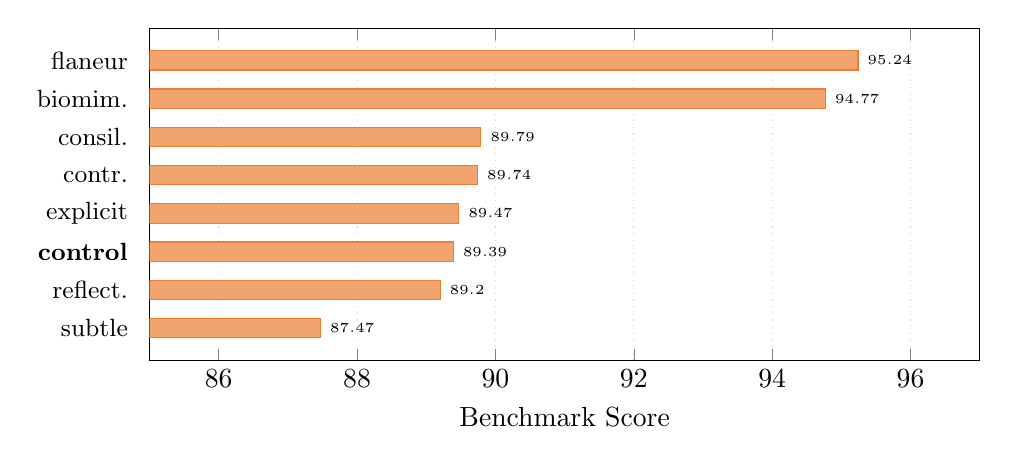
\begin{tikzpicture}
\begin{axis}[
    xbar,
    width=\textwidth,
    height=5.8cm,
    xlabel={Benchmark Score},
    xmin=85, xmax=97,
    symbolic y coords={%
      subtle,reflect.,control,explicit,%
      contr.,consil.,biomim.,flaneur},
    ytick={subtle,reflect.,control,explicit,%
      contr.,consil.,biomim.,flaneur},
    yticklabels={subtle,reflect.,\textbf{control},explicit,%
      contr.,consil.,biomim.,flaneur},
    yticklabel style={font=\small},
    ytick style={draw=none},
    bar width=7pt,
    enlarge y limits=0.12,
    xmajorgrids=true,
    grid style={dotted,gray!40},
    nodes near coords,
    nodes near coords align={horizontal},
    every node near coord/.append style={font=\tiny},
]
\addplot[fill=wikiorange!70, draw=wikiorange]
  coordinates {
    (87.47,subtle)
    (89.20,reflect.)
    (89.39,control)
    (89.47,explicit)
    (89.74,contr.)
    (89.79,consil.)
    (94.77,biomim.)
    (95.24,flaneur)
  };
\end{axis}
\end{tikzpicture}
\subcaption{Aggregate benchmark scores (0--100).  Control baseline in bold.}
\label{fig:benchmark}
\end{minipage}%
\hfill%
\begin{minipage}[t]{0.48\textwidth}
\centering
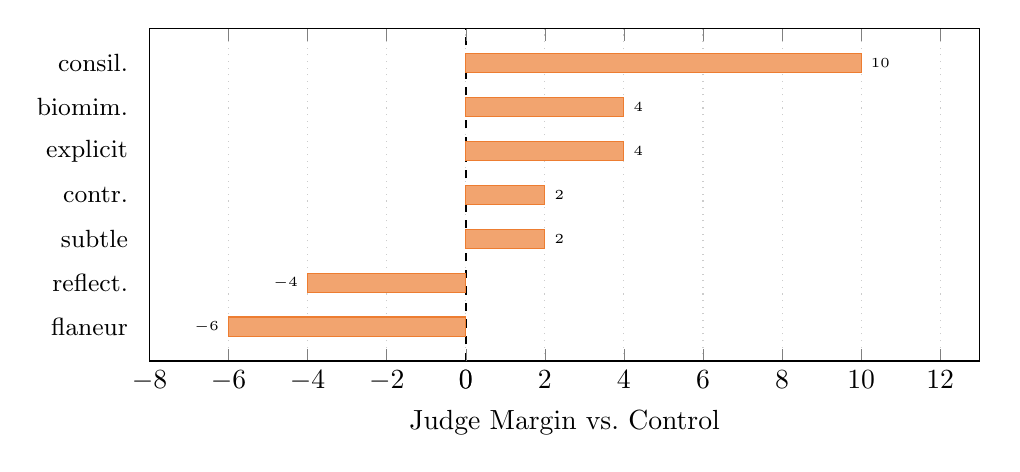
\begin{tikzpicture}
\begin{axis}[
    xbar,
    width=\textwidth,
    height=5.8cm,
    xlabel={Judge Margin vs.\ Control},
    xmin=-8, xmax=13,
    symbolic y coords={%
      flaneur,reflect.,subtle,contr.,%
      explicit,biomim.,consil.},
    ytick=data,
    yticklabel style={font=\small},
    ytick style={draw=none},
    bar width=7pt,
    enlarge y limits=0.13,
    xmajorgrids=true,
    grid style={dotted,gray!40},
    nodes near coords,
    nodes near coords align={horizontal},
    every node near coord/.append style={font=\tiny},
    extra x ticks={0},
    extra x tick style={grid=major, grid style={black,thick,dashed}},
]
\addplot[fill=wikiorange!70, draw=wikiorange]
  coordinates {
    (-6,flaneur)
    (-4,reflect.)
    (2,subtle)
    (2,contr.)
    (4,explicit)
    (4,biomim.)
    (10,consil.)
  };
\end{axis}
\end{tikzpicture}
\subcaption{Blinded LLM judge margin vs.\ control (out of 110).
Positive = Wikipedia condition wins.}
\label{fig:judge}
\end{minipage}
\caption{Benchmark scores (left) and judge margins (right).  The two
measures diverge sharply: flaneur ranks 1st on benchmarks but loses to
control on the judge ($-6$).  Consilience ranks 3rd on benchmarks but
wins the largest judge margin ($+10$).}
\label{fig:bars}
\end{figure*}

% ── 3.2  Scenario Heatmap ───────────────────────────────
\subsection{Scenario Heatmap}

Table~\ref{tab:heatmap} shows per-scenario scores for all conditions,
sorted by aggregate rank.  The top two conditions dominate the same
scenarios: cascading failure (flaneur 1.00, biomimetic 0.98) and
asymmetric routing (flaneur 1.00, biomimetic 0.99).  These are the
scenarios where the middle pack struggles most---control scores 0.87 and
0.85 respectively.  Degradation detection also separates the leaders
(flaneur 1.00, biomimetic 0.99) from control (0.85).  Recovery smoothness
is the most uniform scenario, with all conditions scoring 0.80--0.85.

Two conditions show notably weak asymmetric routing: consilience (0.52)
and explicit (0.53).  Both use weighted-random selection that distributes
load roughly evenly regardless of backend speed---a failure mode that
costs them on this scenario but is masked by strong performance elsewhere.

\begin{table*}[t]
\centering\small
\caption{Per-scenario benchmark scores (0.0--1.0), sorted by aggregate
rank.  Color key:
\colorbox{hcA!30}{$\geq$\,0.90}\;\;%
\colorbox{hcB!40}{0.80--0.89}\;\;%
\colorbox{hcC!60}{0.70--0.79}\;\;%
\colorbox{hcD!50}{0.50--0.69}\;\;%
\colorbox{hcE!50}{$<$\,0.50}.}
\label{tab:heatmap}
\begin{tabular}{@{}l*{7}{c}r@{}}
\toprule
& \textbf{Steady} & \textbf{Degrade} & \textbf{Priority}
& \textbf{Recovery} & \textbf{Cascade} & \textbf{Flapping}
& \textbf{Asymm.} & \textbf{Agg.} \\
& \footnotesize{(w\,=\,1.0)} & \footnotesize{(w\,=\,2.0)}
& \footnotesize{(w\,=\,3.0)} & \footnotesize{(w\,=\,2.0)}
& \footnotesize{(w\,=\,2.0)} & \footnotesize{(w\,=\,1.5)}
& \footnotesize{(w\,=\,1.0)} & \\
\midrule
flaneur      & \hc{0.95} & \hc{1.00} & \hc{1.00} & \hc{0.85}
             & \hc{1.00} & \hc{0.84} & \hc{1.00} & 95.24 \\
biomimetic   & \hc{0.97} & \hc{0.99} & \hc{1.00} & \hc{0.84}
             & \hc{0.98} & \hc{0.84} & \hc{0.99} & 94.77 \\
consilience  & \hc{0.97} & \hc{0.96} & \hc{0.96} & \hc{0.81}
             & \hc{0.96} & \hc{0.91} & \hc{0.52} & 89.79 \\
contrarian   & \hc{0.95} & \hc{0.94} & \hc{0.99} & \hc{0.83}
             & \hc{0.88} & \hc{0.82} & \hc{0.79} & 89.74 \\
explicit     & \hc{0.97} & \hc{0.92} & \hc{0.99} & \hc{0.83}
             & \hc{0.93} & \hc{0.90} & \hc{0.53} & 89.47 \\
control      & \hc{1.00} & \hc{0.85} & \hc{0.96} & \hc{0.83}
             & \hc{0.87} & \hc{0.90} & \hc{0.85} & 89.39 \\
reflective   & \hc{0.96} & \hc{0.90} & \hc{0.99} & \hc{0.83}
             & \hc{0.86} & \hc{0.83} & \hc{0.80} & 89.20 \\
subtle       & \hc{1.00} & \hc{0.83} & \hc{0.98} & \hc{0.80}
             & \hc{0.82} & \hc{0.87} & \hc{0.77} & 87.47 \\
\bottomrule
\end{tabular}
\end{table*}

% ── 3.3  Judge Rankings ──────────────────────────────────
\subsection{Judge Rankings}

Figure~\ref{fig:judge} shows the blinded LLM judge margin for each
condition versus control.  Consilience achieves the largest margin ($+10$
points), with the judge praising its AIMD recovery model, weighted-random
selection for proportional degradation, and data-driven shed tiers.
Biomimetic and explicit tie at $+4$.  Contrarian and subtle each win by
$+2$.

Two conditions \emph{lose} to control: reflective ($-4$) and flaneur
($-6$).  The judge found real code-quality issues in flaneur---a
mislabeled routing function and a no-op recovery transition---that do not
affect benchmark scores but reflect lower design clarity.  Control scored
between 60 and 68 across its seven pairings, introducing meaningful noise
in the margins.

% ── 3.4  Judge vs Benchmark Divergence ───────────────────
\subsection{Judge vs.\ Benchmark Divergence}
\label{sec:divergence}

The judge and benchmark diverge more dramatically than in previous work.
The most striking case:

\begin{itemize}
\item \textbf{Flaneur}: Benchmark rank 1st (95.24); Judge margin $-6$
  (control wins).  The benchmark rewards flaneur's near-perfect cascading
  failure isolation (1.00) and asymmetric routing (1.00).  The judge
  penalizes code-quality issues and awards no cross-domain insight
  credit---because flaneur's research was on-topic, not cross-domain.
\item \textbf{Consilience}: Benchmark rank 3rd (89.79, within 0.4 of
  control); Judge rank 1st ($+10$ margin).  The judge praised AIMD
  recovery and weighted-random selection.  The benchmark shows consilience
  is dragged down by poor asymmetric routing (0.52)---its weighted-random
  selection ignores backend speed.
\item \textbf{Subtle}: Benchmark rank 8th (87.47); Judge margin $+2$.
  The judge slightly preferred subtle's smooth weighted round-robin, but
  the benchmark penalizes its slower degradation detection (0.83) and
  weaker cascading failure handling (0.82).
\end{itemize}

The judge evaluates architecture and design reasoning.  The benchmark
evaluates whether the code works under fault injection.  Each captures a
different dimension of quality, and they can disagree sharply on the same
implementation.

% ── 3.5  Cost and Efficiency ─────────────────────────────
\subsection{Cost and Efficiency}

Figure~\ref{fig:cost} plots benchmark score against API cost.
Table~\ref{tab:efficiency} shows the full breakdown.  Subtle is the
cheapest overall (\$0.68, 3:03) but scores lowest.  Control is the
most cost-efficient at \$1.43 for 89.39 points (62.5 score/\$).
Among Wikipedia conditions, flaneur achieves the best
return---\$1.94 for 95.24 points (49.1 score/\$), the cheapest
research condition and the highest score.  Biomimetic costs
\$3.96 for 94.77 points.  Consilience is the most
expensive at \$4.01 for only 0.4 points above control.

Research time dominates cost for most conditions.  Flaneur's research
completed in 426 seconds with 37 retrieval turns---the fastest
research condition.  Consilience's research took 1,275 seconds
with 79 turns and 769 seconds of synthesis, reflecting its instruction
to find convergent patterns across five or more domains.

\begin{table}[H]
\centering\small
\caption{Cost, efficiency, and code metrics.  Score/\$ = benchmark score
per dollar of API cost.  Research time includes retrieval and synthesis.}
\label{tab:efficiency}
\begin{tabular}{@{}lrrrrr@{}}
\toprule
\textbf{Condition} & \textbf{Time} & \textbf{Cost}
  & \textbf{LOC} & \textbf{Res.}  & \textbf{Sc./\$} \\
\midrule
subtle      & 3:03  & \$0.68 & 407 &  ---  & 128.6 \\
control     & 7:48  & \$1.43 & 414 &  ---  &  62.5 \\
flaneur     & 9:45  & \$1.94 & 446 &  7:06 &  49.1 \\
reflective  & 12:06 & \$2.55 & 428 &  8:42 &  35.0 \\
explicit    & 13:52 & \$2.65 & 543 &  8:53 &  33.8 \\
contrarian  & 14:02 & \$3.05 & 530 & 10:11 &  29.4 \\
biomimetic  & 20:14 & \$3.96 & 728 & 11:58 &  23.9 \\
consilience & 31:09 & \$4.01 & 437 & 21:15 &  22.4 \\
\bottomrule
\end{tabular}
\end{table}

% ── 3.6  Wikipedia Usage ─────────────────────────────────
\subsection{Wikipedia Usage}

Table~\ref{tab:wiki} shows research effort versus knowledge extraction.
Six conditions actively retrieved Wikipedia articles; control and subtle
did not.  All six active conditions read 9--12 articles each---a
narrow range that suggests the retrieval pipeline converges on a
similar volume regardless of persona.

The \emph{content} of the articles varies dramatically.  Biomimetic read
exclusively biological articles (allostasis, homeostasis, apoptosis,
torpor, optimal foraging theory).  Contrarian focused on failure modes
(systemic risk, demand response, C10k problem).  But flaneur---instructed
to random-walk---read fault tolerance, thundering herd problem,
consistent hashing, weighted round-robin, and deficit round-robin.
Every article is directly relevant to load balancing.  The flaneur
\emph{defected from its research persona}, searching on-topic articles
instead of exploring randomly (see Section~\ref{sec:flaneur}).

\begin{table}[H]
\centering\small
\caption{Wikipedia usage per condition.  ``Tokens'' = research subagent
output tokens; ``Articles'' = articles read from retrieval manifest.}
\label{tab:wiki}
\begin{tabular}{@{}lrrp{2.5cm}@{}}
\toprule
\textbf{Cond.} & \textbf{Tokens} & \textbf{Art.}
  & \textbf{Key Sources} \\
\midrule
control     &     0 &  0 & --- \\
subtle      &     0 &  0 & Tools not discovered \\
explicit    & 5,101 & 11 & Load shedding, DiffServ \\
reflective  & 3,832 & 11 & Circuit breaker, C10k \\
flaneur     & 7,052 &  9 & Fault tolerance, WRR \\
consilience & 4,814 & 12 & TCP cong., HRA \\
biomimetic  & 6,892 &  9 & Allostasis, torpor \\
contrarian  & 6,088 &  9 & Systemic risk, C10k \\
\bottomrule
\end{tabular}
\end{table}

\begin{figure*}[t]
\centering
\begin{minipage}[t]{0.48\textwidth}
\centering
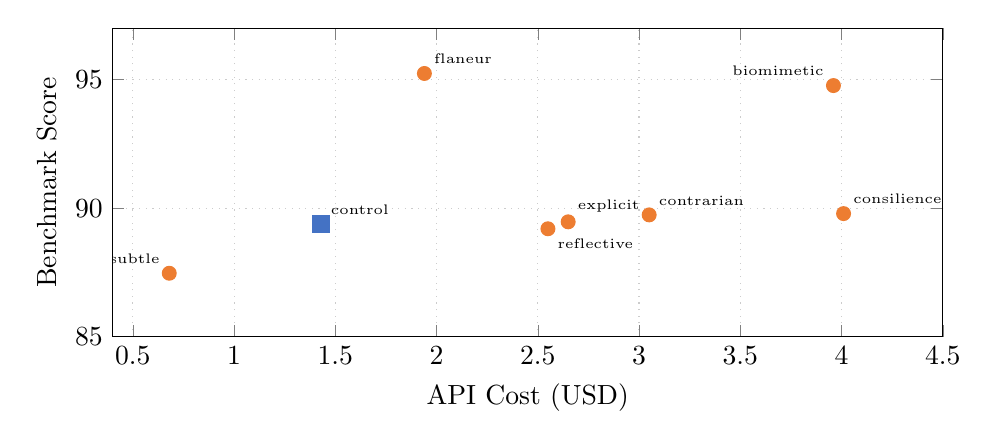
\begin{tikzpicture}
\begin{axis}[
    width=\textwidth,
    height=5.5cm,
    xlabel={API Cost (USD)},
    ylabel={Benchmark Score},
    xmin=0.4, xmax=4.5,
    ymin=85, ymax=97,
    grid=major,
    grid style={dotted,gray!40},
    only marks,
    mark size=2.5pt,
]
% Control point (blue square)
\addplot[controlblue, mark=square*, mark size=3pt]
  coordinates {(1.43,89.39)};
% Wiki points (orange circles)
\addplot[wikiorange, mark=*, mark size=2.5pt]
  coordinates {
    (0.68,87.47)
    (2.65,89.47)
    (2.55,89.20)
    (1.94,95.24)
    (4.01,89.79)
    (3.96,94.77)
    (3.05,89.74)
  };
% Labels
\node[font=\tiny, anchor=south west] at (axis cs:1.43,89.39) {control};
\node[font=\tiny, anchor=south east] at (axis cs:0.68,87.47) {subtle};
\node[font=\tiny, anchor=south west] at (axis cs:2.65,89.47) {explicit};
\node[font=\tiny, anchor=north west] at (axis cs:2.55,89.20) {reflective};
\node[font=\tiny, anchor=south west] at (axis cs:1.94,95.24) {flaneur};
\node[font=\tiny, anchor=south west] at (axis cs:4.01,89.79) {consilience};
\node[font=\tiny, anchor=south east] at (axis cs:3.96,94.77) {biomimetic};
\node[font=\tiny, anchor=south west] at (axis cs:3.05,89.74) {contrarian};
\end{axis}
\end{tikzpicture}
\subcaption{Benchmark score vs.\ API cost.  Control (blue square);
flaneur delivers the highest score at 1.4$\times$ control's cost.}
\label{fig:cost}
\end{minipage}%
\hfill%
\begin{minipage}[t]{0.48\textwidth}
\centering
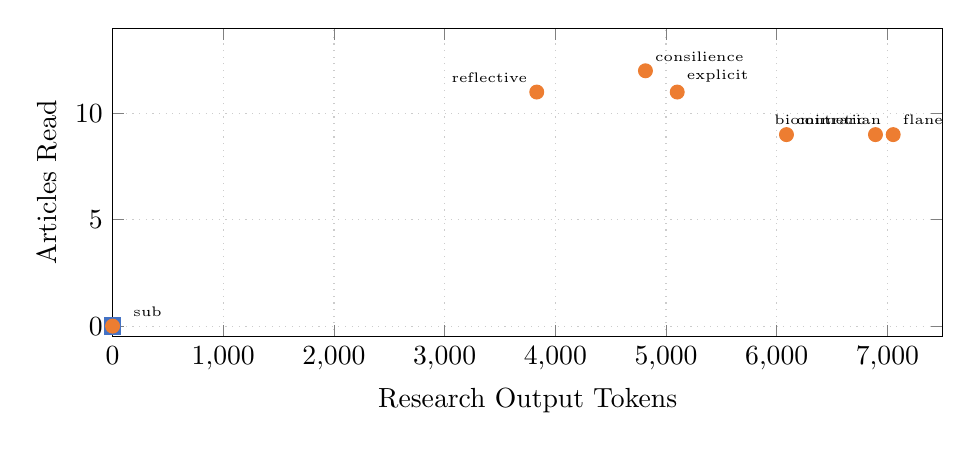
\begin{tikzpicture}
\begin{axis}[
    width=\textwidth,
    height=5.5cm,
    xlabel={Research Output Tokens},
    ylabel={Articles Read},
    xmin=0, xmax=7500,
    ymin=-0.5, ymax=14,
    grid=major,
    grid style={dotted,gray!40},
    only marks,
    mark size=2.5pt,
]
% Control + subtle (no research)
\addplot[controlblue, mark=square*, mark size=3pt]
  coordinates {(0,0)};
% Wiki points (orange circles)
\addplot[wikiorange, mark=*, mark size=2.5pt]
  coordinates {
    (0,0)
    (5101,11)
    (3832,11)
    (7052,9)
    (4814,12)
    (6892,9)
    (6088,9)
  };
% Labels
\node[font=\tiny, anchor=south east] at (axis cs:0,0) {ctrl};
\node[font=\tiny, anchor=south west] at (axis cs:100,0) {sub};
\node[font=\tiny, anchor=south west] at (axis cs:5101,11) {explicit};
\node[font=\tiny, anchor=south east] at (axis cs:3832,11) {reflective};
\node[font=\tiny, anchor=south west] at (axis cs:7052,9) {flaneur};
\node[font=\tiny, anchor=south west] at (axis cs:4814,12) {consilience};
\node[font=\tiny, anchor=south east] at (axis cs:6892,9) {biomimetic};
\node[font=\tiny, anchor=south west] at (axis cs:6088,9) {contrarian};
\end{axis}
\end{tikzpicture}
\subcaption{Research effort vs.\ knowledge extraction.  All active
conditions read 9--12 articles; token usage varies 2$\times$.}
\label{fig:wiki}
\end{minipage}
\caption{Cost--performance trade-off (left) and Wikipedia research
patterns (right).}
\label{fig:scatters}
\end{figure*}

\FloatBarrier

% ─────────────────────────────────────────────────────────
% 4. WHAT EACH AGENT BUILT
% ─────────────────────────────────────────────────────────
\section{What Each Agent Built}

Table~\ref{tab:arch} summarizes the architectural choices made by each
condition.  Despite identical problem specifications, the eight agents
produced meaningfully different designs.

\begin{table*}[t]
\centering\small
\caption{Architectural comparison across conditions.  WLC = weighted
least-connections; WRR = weighted round-robin; SWRR = smooth weighted
round-robin; AIMD = additive increase / multiplicative decrease;
EMA/EWMA = (exponential) weighted moving average.}
\label{tab:arch}
\begin{tabular}{@{}lllllr@{}}
\toprule
\textbf{Condition} & \textbf{Routing} & \textbf{Health Tracking}
  & \textbf{Shedding} & \textbf{Recovery} & \textbf{LOC} \\
\midrule
control     & WLC             & EMA ($\alpha{=}0.4$)
  & Priority tiers            & Asym.\ ramp ($+$0.15/$-$0.4)  & 414 \\
flaneur     & Weighted RR     & EWMA + synthetic latency
  & Demand-response           & No-volt release ($\times$0.5/$+$0.10) & 446 \\
biomimetic  & Foraging (E/h)  & Trail pheromone EMA
  & Allostatic redistrib.     & 4-state torpor machine & 728 \\
consilience & Weighted random  & AIMD weight
  & Tiered escalation         & Probe-gated ($+$0.05) & 437 \\
contrarian  & Weighted LC      & EMA + latency tiers
  & Multi-stage UFLS          & AIMD ($\times$0.5/$+$0.05)    & 530 \\
explicit    & Weighted random  & Graduated continuous
  & Capacity-coupled          & Linear ($+$0.05)      & 543 \\
reflective  & SWRR (Nginx)    & EMA + sliding window
  & Priority tiers            & Asym.\ ramp ($+$0.15/$-$0.3)  & 428 \\
subtle      & WLC             & Graduated continuous
  & Staged tiers              & Asym.\ ramp ($+$0.15/$-$0.4)  & 407 \\
\bottomrule
\end{tabular}
\end{table*}

\textbf{Control} (414~LOC) implements weighted least-connections routing
with EMA health tracking ($\alpha{=}0.4$).  Priority-based shedding
activates at fixed capacity thresholds (background$<$70\%, normal$<$40\%,
critical$<$15\%).  An asymmetric weight ramp ($+$0.15/tick up,
$-$0.4/tick down) prevents thundering herd on recovery.  A solid,
conventional baseline.

\textbf{Flaneur} (446~LOC) uses weighted round-robin with a scoring
function: \texttt{weight/(1+avg\_latency/100)}, normalizing latency
relative to a 100ms baseline.  Failed requests inject a synthetic 500ms
latency penalty into the EMA, making health tracking highly responsive.
Its ``no-volt release'' recovery---fast ramp-down ($\times$0.5) and slow
ramp-up ($+$0.10/tick)---mirrors power-grid demand-response patterns.
The implementation excels at cascading failure (1.00) and asymmetric
routing (1.00) because latency-weighted scoring naturally routes away from
slow backends.

\textbf{Biomimetic} (728~LOC) is the most architecturally distinctive.
Routing uses optimal foraging theory: each backend's ``profitability''
is health/latency (energy per handling time), and the router selects from
the top-50\% profitability tier.  A four-state machine
(HEALTHY$\to$DEGRADED$\to$TORPID$\to$RECOVERING) governs backend
lifecycle---torpid backends receive probes only, and recovery caps
requests at \texttt{max(1, round(progress$\times$5))}.  This is the only
condition where biological analogies produced structural---not merely
terminological---differences in the architecture.

\textbf{Consilience} (437~LOC) implements AIMD-based weighted random
selection.  Multiplicative decrease ($\times$0.5) on failure, additive
increase ($+$0.05/tick) on recovery, but recovery is gated through probes:
only probe outcomes trigger additive increase, rate-limiting recovery to
one tick at a time.  Despite referencing five convergent patterns
(TCP congestion, power-grid UFLS, ALOHA, high-redundancy actuation,
DiffServ), its asymmetric routing fails (0.52)---weighted-random
distributes load evenly regardless of backend speed.

\textbf{Contrarian} (530~LOC) combines weighted-random routing with
active-request tracking (a least-connections variant).  Multi-tier latency
sensitivity distinguishes ``degraded'' (300ms) from ``severe'' (800ms)
with different multiplicative decreases.  Its multi-stage shedding
escalates through four thresholds.  The adversarial research strategy
produced careful fault detection but no structural innovation.

\textbf{Explicit} (543~LOC) implements weighted-random selection with
graduated continuous health scoring---latency is linearly interpolated
between 50ms (healthy) and 500ms (failed), avoiding binary
up/down decisions.  Linear recovery ($+$0.05/tick) avoids oscillation
in small-$N$ deployments.

\textbf{Reflective} (428~LOC) uses smooth weighted round-robin
(Nginx's SWRR algorithm), the only condition with deterministic
routing.  A three-state enum (HEALTHY/DEGRADED/UNHEALTHY) with
dual-threshold transitions provides clean state management.

\textbf{Subtle} (407~LOC) is architecturally near-identical to control:
weighted least-connections with graduated health scoring and staged
shedding.  It never discovered the Wikipedia tools during its run,
confirming the retrieval manifest's zero-article record.

% ─────────────────────────────────────────────────────────
% 5. DISCUSSION
% ─────────────────────────────────────────────────────────
\section{Discussion}

Six observations emerge from this experiment.

\textbf{1.\ Cross-domain research can improve functional benchmarks
by ${\sim}6$ points---but the effect is concentrated.}  Flaneur and
biomimetic score 5--6 points above control, but the gap comes almost
entirely from three scenarios: cascading failure, asymmetric routing,
and degradation detection.  On recovery, priority protection, and
flapping, they perform comparably to the middle pack.  The improvement
is real but narrow---specific failure scenarios where latency-aware or
profitability-based routing excels, not a general quality lift.

\textbf{2.\ The flaneur defected from its instructions---and this is
the most interesting finding.}
\label{sec:flaneur}
The flaneur was instructed to ``take a random walk through Wikipedia; let
connections emerge.''  Its retrieval manifest shows it read: fault
tolerance, thundering herd problem, exponential backoff, consistent
hashing, weighted round-robin.  Every article is directly relevant to load
balancing.  The agent ignored its creative persona and searched for what
it already knew was relevant.

This is simultaneously an \emph{apparatus flaw} and a \emph{finding
about agent behavior}.  As an apparatus flaw: we cannot claim the flaneur
condition tests undirected exploration, because undirected exploration
didn't happen.  As a behavioral finding: when an LLM agent is given a
creative research instruction but knows the problem domain, it
gravitates toward on-topic material.  The retrieval verification catches
\emph{whether} articles were read, not \emph{how} they were found.
Enforcing research strategy---as opposed to research access---is an open
problem for agent experiment design.

\textbf{3.\ Biomimetic is the only genuine cross-domain success.}
Of the seven Wikipedia conditions, biomimetic is the only one that
(a) followed its cross-domain research instructions (reading articles on
allostasis, homeostasis, apoptosis, torpor, and optimal foraging theory),
(b) produced a structurally distinct architecture (four-state torpor
machine, foraging-profitability routing), and (c) scored well on
benchmarks (94.77, rank 2).  However, it is also the most
expensive (\$3.96, 2.8$\times$ control) and produced the most code
(728 LOC vs.\ 414 control).  The structural translation from biological
concepts to software design appears to require significant additional
compute.

\textbf{4.\ The judge and benchmark measure orthogonal things.}
The flaneur divergence is the starkest example: benchmark rank~1st,
judge rank~last ($-6$).  But the pattern extends further.  Consilience
wins the largest judge margin ($+10$) while sitting at 89.79 on the
benchmark---0.4 points from control.  The judge rewards architectural
ambition, cross-domain insight, and design reasoning.  The benchmark
rewards whether the code actually isolates failures and routes
traffic correctly.  Neither is wrong, but for production evaluation,
\emph{behavioral benchmarks should take precedence}---a load balancer
that isolates cascading failures matters more than one the judge finds
architecturally interesting.

\textbf{5.\ The middle pack is noise.}  Five conditions
(consilience, contrarian, explicit, control, reflective) cluster in a
0.6-point band from 89.20 to 89.79.  With $N{=}1$ per condition, we
cannot distinguish this from variance.  The experiment has statistical
power to detect flaneur and biomimetic's ${\sim}6$-point gap but cannot
make meaningful claims about conditions separated by less than a point.

\textbf{6.\ The compute-time confound is real but not decisive.}
Research conditions consume 3--31 minutes of total time versus
control's 8 minutes.  However, flaneur's \emph{coding} stage took only
159 seconds---less than subtle (183s) and far less than control
(468s)---yet produced the highest score.  Biomimetic's coding stage
(496s) was comparable to control's.  The confound is real---more total
compute is available---but the coding-time data suggests the research
\emph{content}, not merely the extra thinking time, drives the effect
for the top two conditions.

\paragraph{Limitations.}
This is a single-problem ($N{=}1$), single-model (Claude), single-judge
experiment.  Each condition was run once, so we cannot estimate
within-condition variance.  The LLM judge's control scores varied
between 60 and 68 across seven pairings, introducing noise in the
margin estimates.  The flaneur defection means we tested six research
personas, not seven---the flaneur result is interesting but does not
test undirected exploration as designed.  Parametric knowledge
contamination means Wikipedia may be reinforcing what the model already
knows rather than introducing genuinely new information.

% ─────────────────────────────────────────────────────────
% 6. CONCLUSION
% ─────────────────────────────────────────────────────────
\enlargethispage{2\baselineskip}
\section{Conclusion}

Wikipedia access can improve LLM-generated code, but the effect is
narrower and more conditional than a headline score suggests.  Two of
seven Wikipedia conditions clearly outperformed control---flaneur by 5.85
points and biomimetic by 5.38---while five clustered within 0.6 points of
the baseline.  The improvement concentrates in specific failure scenarios
(cascading failure, asymmetric routing, degradation detection), not a
general quality lift.

The experiment's most interesting finding may be its flaws.  The flaneur
did not random-walk---it searched on-topic.  The subtle condition did not
discover its tools.  The judge and benchmark disagree sharply on the
same code.  These failures expose real challenges in agent experiment
design: enforcing research strategy compliance, separating Wikipedia's
contribution from parametric knowledge, and choosing evaluation methods
that align with the quality dimensions that matter.

Biomimetic stands out as the only condition that followed its cross-domain
instructions, produced a structurally distinct architecture, and scored
well---suggesting that when structural translation from another domain
actually happens, the results can be meaningful.  Whether this transfers
to other problem types, at larger $N$, remains an open question.

\end{document}
